\chapter{Магнитное поле в веществе}

\section{Намагничивание вещества}

    Все до единого вещества при помещении их в магнитное поле каким-либо образом
    искажают его и взаимодействуют с ним: втягиваются или выталкиваются.
    
    \begin{figure}[!b]
        \center
        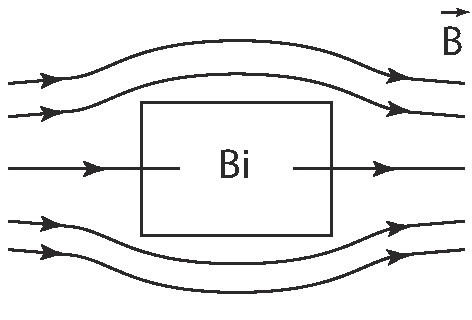
\includegraphics[width=0.3\linewidth]{lec09/bismuthum.pdf}
        \hfill
        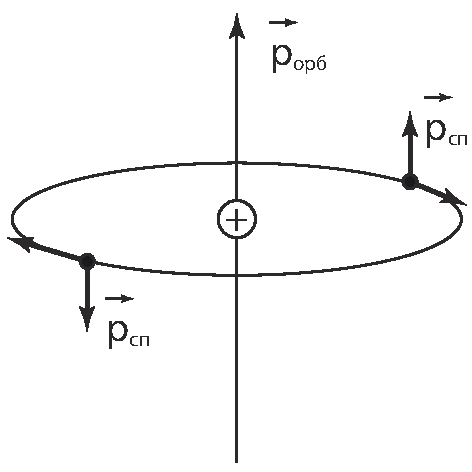
\includegraphics[width=0.3\textwidth]{lec09/atom_moment.pdf}
        \parbox[t]{.47\textwidth}{\caption{Висмут -- пример типичного
            диамагнетика}}
        \hfill
        \parbox[t]{.47\textwidth}{\caption{Природа намагниченности}}
    \end{figure}

    Это означает, что все вещества являются магнетиками, то есть способны
    индуцировать собственный магнитный момент в поле \( \vec{B} \). Появление
    магнитного момента у всех веществ объясняется атомарной структурой. Средний
    магнитный момент атома складывается из двух компонент -- орбитальной и
    спиновой:
    \[
        \midnum{\vec{p}_m}=\sum\vec{p}_\textit{орбит}+\sum\vec{p}_\textit{спин}.
    \]
    
    \begin{definition}
        Магнитный момент единицы объема вещества называется 
        \textbf{намагниченностью} вещества.
    \end{definition}
    Таким образом, вектор намагниченности \( \vec{M} \) определяется так:
    \[
        \vec{M} = \frac{\sum \vec{p}_m}{\Delta V} =
        \frac{N}{\Delta V}\midnum{\vec{p}_m} = n\midnum{\vec{p}_m}.
    \]
    В зависимости от химического состава и структуры вещества существует
    несколько механизмов намагничивания.
    
\section{Механизмы намагничивания слабомагнитных веществ}
    Все вещества по механизму намагничивания делятся на три группы:
    \begin{itemize}
    \item
        парамагнетики;
    \item
        диамагнетики;
    \item
        ферромагнетики.
    \end{itemize}
    
    Парамагнетики и диамагнетики являются \textit{слабомагнитыми} веществами, а
    ферромагнетики -- \textit{сильномагнитными}.
    
\subsection{Парамагнетики}
    \textbf{Парамагнетики} -- это вещества, молекулы которых имеют собственный
    ненулевой магнитный момент даже в отсутствие внешнего поля \( \vec{B} \)
    \[
        \midnum{\vec{p}_m} = \sum\vec{p}_{\textit{орбит}} +
        \sum\vec{p}_{\textit{спин}} \ne 0.
    \]
    Однако в целом образец магнитно нейтрален, то есть
    \[
        \sum \midnum{\vec{p}_m} = 0,
    \]
    так как все элементарные магнитные моменты ориентированы хаотично. При
    наложении внешнего поля \( \vec{B} \) эти элементарные магнитные диполи
    \textit{слегка} упорядочиваются, и образец намагничивается:
    \[
        \sum \midnum{\vec{p}_m} \ne 0 \Rightarrow \vec{M} \ne 0.
    \]
    
    \begin{figure}[h]
        \center
        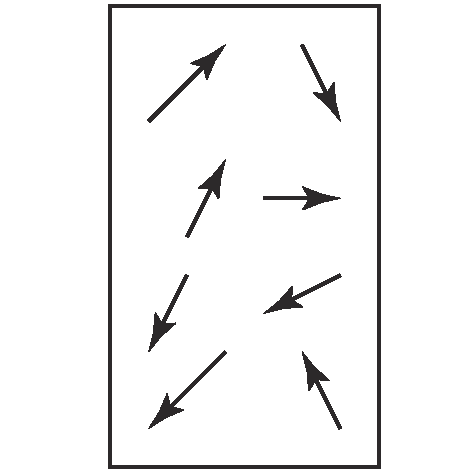
\includegraphics[width=.47\textwidth]{lec09/para_wo_B.pdf}
        \hfill
        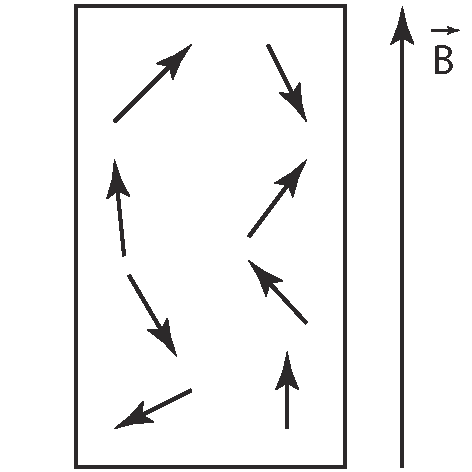
\includegraphics[width=.47\textwidth]{lec09/para_in_B.pdf}
        \parbox[t]{.47\textwidth}{\caption{Парамагнетик в отсутствие внешнего
            поля не обладает намагниченностью}}
        \hfill
        \parbox[t]{.47\textwidth}{\caption{При помещении его во внешнее поле
            магнитные моменты его атомом в слегка выстраиваются и появляется
            небольшая намагниченность}}
    \end{figure} 

    К парамагнетикам относятся такие вещества, как \( Al, Pt, O_2, NO, MnO,
    FeCl_2 \). Парамагнетики втягиваются в область более сильного поля.
    
\subsection{Диамагнетики}
    \begin{figure}[b!]
        \center
        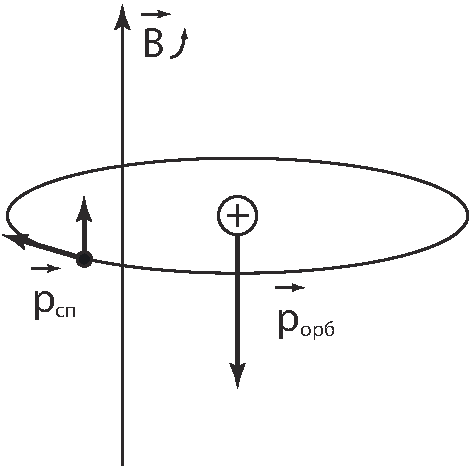
\includegraphics[width=.47\textwidth]{lec09/diamagnetic.pdf}
        \caption{Поведение диамагнетика при его внесении во внешнее поле}
    \end{figure} 
    \textbf{Диамагнетики} -- это вещества, молекулы которых не имеют
    собственного магнитного момента:
    \[
        \midnum{\vec{p}_m} = \sum\vec{p}_{\textit{орбит}} +
        \sum\vec{p}_{\textit{спин}} = 0.
    \]
    Однако, при наложении внешнего поля \( \vec{B} \) эти моменты индуцируются,
    причем они направлены против поля \( \vec{B} \). Механизм диамагнетизма
    связан с правилом Ленца %(см. п~\ref{sec:11:1}).
    
    По правилу Ленца, магнитный поток через сечение орбиты электрона не должен
    меняться. А так как поле \( \vec{B} \) возрастает, то скорость электрона так
    же увеличивается, чтобы \( \Delta\vec{B}_{\textit{собств}} +
    \Delta\vec{B}_{\textit{внеш}} = 0 \). Поэтому \( \vec{M} \uparrow\downarrow
    \vec{B}_{\textit{внеш}} \).
    
    Характерными представителями диамагнетиков являются \( Bi, Cu, Sn, S, H_2O
    \). В противоположность парамагнетикам, диамагнетики выталкиваются из поля.
    
    Особенностью всех слабомагнитных веществ является обратимость
    намагниченности, то есть при снятии поля \( \vec{B} \) намагниченность
    исчезает.
    
\section{Магнитное поле в веществе}

    Индуцируемое молекулярными токами \( i’ \) поле \( \vec{B}{’} \),
    складываясь с внешним полем \( \vec{B}_0 \), и дает результирующее поле 
    \[
        \vec{B} = \vec{B}_0 + \vec{B}{’},
    \]
    которое и является магнитным полем в веществе и окружающем его пространстве.
    А так как индуцированное поле \( \vec{B}{’} \) порождается движущимися
    зарядами, то
    \[
        \div\vec{B}{’} = 0,
    \]
    и, следовательно,
    \[
        \div\vec{B} = \div\vec{B}_0 + \div\vec{B}{’} = 0.
    \]
    
\section{Вектор \textbf{H} и его циркуляция}

    Запишем циркуляцию вектора \( \vec{B} \):
    \begin{equation}
        \oint\limits_C \vec{B}\cdot\dd\vec{l} = \mu_0(i’ + i)_C,
        \label{eq9:1}
    \end{equation}
    где \( i_C \) -- суммарный свободный ток, охватываемый контуром \( C \),
    \( i’_C \) -- суммарный молекулярный ток, охватываемый контуром \( C \).
        \begin{figure}[b!]
            \center
            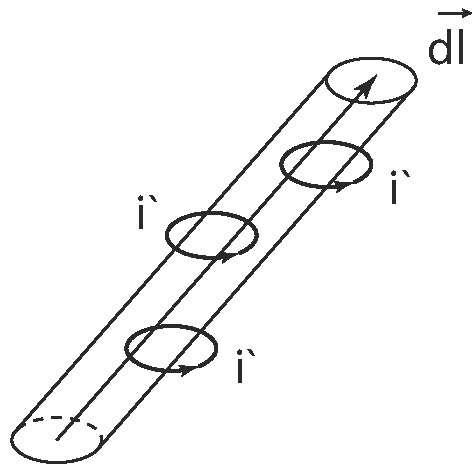
\includegraphics[width=0.3\textwidth]{lec09/circulation_H.pdf}
            \caption{К вычислению поля \( \vec{H} \)}
        \end{figure}
    Вычислим \( i’_C \) и выразим его через \( \vec{M} \). Для этого выделим
    малый элемент контура \( \dd\vec{l} \) и посчитаем суммарный молекулярный
    ток, нанизанный на него. Элемент \( \dd\vec{l} \) пронизывают только те
    молекулярные токи, центры которых лежат в косом цилиндре (\(S’, \dd l\)).
    Тогда суммарный молекулярный ток в этом цилиндре \( \dd i’ = i’\dd N \),
    где \( \dd N \) -- число молекулярных токов в цилиндре (\(S’, \dd l\)).
    Объем цилиндра \( \dd V = S’\dd l\cos\alpha \).
    
    Тогда суммарный молекулярный ток в косом цилиндре:
    \[
        \dd i’ = ni’\dd V = ni’S’\dd l\cos\alpha,
    \]
    а так как \( i’S’ = \midnum{p_m} \) -- средний молекулярный магнитный
    момент, то
    \[
        \dd i’ = n\midnum{p_m}\dd l\cos\alpha,
    \]
    а по определению \( \vec{M} = n\midnum{\vec{p}_m} \). Следовательно,
    \[
        \dd i’ = M\dd l\cos\alpha = \vec{M}\cdot\dd\vec{l}.
    \]
    Интегрируя по всему контуру \( C \), получим
    \begin{equation}
        i’_C = \oint\limits_C \vec{M}\cdot\dd\vec{l}.
        \label{eq9:2}
    \end{equation}
    
    Формула (\ref{eq9:2}) выражает теорему о циркуляции вектора \( \vec{M} \).
    Подставив (\ref{eq9:2}) в (\ref{eq9:1}), получим
    \[
        \oint\limits_C \left(\frac{\vec{B}}{\mu_0} -
        \vec{M}\right)\cdot\dd\vec{l} = i_C.
    \]
    
    Выражение в скобках обозначается через \( \vec{H} \):
    \begin{equation}
        \vec{H} = \frac{\vec{B}}{\mu_0} - \vec{M}.
        \label{eq9:3}
    \end{equation}
    
    Тогда теорема о циркуляции вектора \( \vec{H} \):
    \begin{equation}
        \oint\limits_C \vec{H}\cdot\dd\vec{l} = \left(\sum i\right)_C.
        \label{eq9:4}
    \end{equation}

    При непрерывном распределении тока
    \[
        i = \iint\limits_S \vec{j}\cdot\dd\vec{S}.
    \]
    По теореме Стокса
    \[
        \oint\limits_C \vec{H}\cdot\dd\vec{l} =
        \iint\limits_S \rot\vec{H}\cdot\dd\vec{S}.
    \]
    В силу произвольности поверхности \( S \)
    \begin{equation}
        \rot\vec{H} = \vec{j}.
        \label{eq9:4a}
    \end{equation}
    
    Формула (\ref{eq9:4a}) -- дифференциальная форма теоремы о циркуляции
    \( \vec{H} \) (\ref{eq9:4}).
    
\section{Терминология и определения}

    \begin{tabular}[ht]{|c|c|c|c|} \hline
    Величина & Название & Определение & Комментарий \\ \hline
    %-----------------------------------------------------------------
    &&&\\
    \( E \) & Электрическое поле & \( \vec{F} = q\vec{E} \)
    & Основная силовая характеристика \\ &&&\\
    \( P \) & Поляризованность & \( \vec{P} = \frac{1}{\Delta V}\sum\vec{p}_e \)
    & Электрическое состояние вещества \\ &&&\\
    \( D \) & Вектор \( \vec{D} \) & \( \vec{D} = \eps_0\vec{E} + \vec{P} \)
    & Вспомогательная величина \\ &&&\\ \hline
    %-----------------------------------------------------------------
    &&&\\
    \( B \) & Магнитное поле & \( \vec{F} = q(\vec{v}\times\vec{B}) \) 
    & Основная силовая характеристика \\ &&&\\
    \( M \) & Намагниченность & \( \vec{M} = \frac{1}{\Delta V}\sum\vec{p}_m \)
    & Магнитное состояние вещества \\ &&&\\
    \( H \) & Вектор \( \vec{H} \) & \( \vec{H} = \frac{\vec{B}}{\mu_0}
    - \vec{M} \) & Вспомогательная величина \\ &&&\\ \hline
    %-----------------------------------------------------------------
    \end{tabular}
    
\section{Связь между векторами \textbf{M}, \textbf{B} и \textbf{H} у слабомагнитных веществ}

    Для слабомагнитных веществ \( \vec{M} \sim \vec{H} \). Из формулы
    (\ref{eq9:3}) следует, что размерности векторов \( \vec{H} \) и
    \( \vec{M} \) совпадают, поэтому
    \begin{equation}
        \vec{M} = \chi\vec{H}.
        \label{eq9:5}
    \end{equation}

    Коэффициент \( \chi \) в формуле (\ref{eq9:5}) называется \textbf{магнитной 
    восприимчивостью} вещества. Подставляя (\ref{eq9:5}) в (\ref{eq9:3}),
    получим
    \begin{equation}
        \vec{B} = \mu\mu_0\vec{H}.
        \label{eq9:6}
    \end{equation}

    Коэффициент
    \[
    \mu = \chi + 1 
    \]
    называется \textbf{магнитной проницаемостью} вещества. Тогда связь между
    векторами \( \vec{B} \) и \( \vec{M} \)
    \begin{equation}
         \vec{M} = \frac{\chi}{\mu\mu_0}\vec{B}.
         \label{eq9:ololo}
    \end{equation}

    Формулы (\ref{eq9:5}), (\ref{eq9:6}) и (\ref{eq9:ololo}) определяют искомую
    связь между векторами \( \vec{M}, \vec{B} \) и \( \vec{H} \).

\section{Единицы измерения}

    В системе СГСМ
    \[
        [B] = [H] = [M] = \text{Гс (гаусс)} = \text{Э (эрстед)},
    \]
    \[
        \vec{B} = \vec{H} + 4\pi\vec{M}.
    \]

    В СИ
    \[
        [B] = \text{Тл (тесла)}; [H] = [M] = \frac{\text{А}}{\text{м}}.
    \]
    \[
        1 \text{Тл} = 10^4 \text{Гс} = 10 \text{кГс}.
    \]

    Так как в вакууме \( \vec{B} = \mu_0\vec{H} \), то при \( B = 1 \)Тл 
    \( H \approx 8 \times 10^5 \frac{\text{А}}{\text{м}} \).

\section{Граничные условия}

    Пусть два вещества \( \mu_1 \) и \( \mu_2 \), имеющие общую границу раздела,
    помещены в поле \( \vec{B} \). Так как \( \vec{B} = \mu\mu_0\vec{H} \), то
    в любой точке \( \vec{B} \uparrow\uparrow \vec{H} \). Установим характер
    преломления линий полей \( \vec{B} \) и \( \vec{H} \) на границе.

    Теорема Гаусса для поля \( \vec{B} \):
    \[
        \oiint\limits_S \vec{B}\cdot\dd\vec{S} = 0.
    \]
    Охватим участок границы цилиндрической поверхностью малой высоты
    \( h \ll \sqrt{S_{\textit{тор}}} \). Тогда, по теореме Гаусса:
    \[
        \oiint\limits_S \vec{B}\cdot\dd\vec{S} = 
        -B_{n1}S_{\textit{тор}}^{\text{верх}} + 
        B_{n2}S_{\textit{тор}}^{\text{ниж}} = 0.
    \]
    
    А так как \( S_\textit{тор}^\text{верх} = S_\textit{тор}^\text{ниж} \), то
    \begin{equation}
        B_{n1} = B_{n2}
        \label{eq9:n1}
    \end{equation}
    Уравнение (\ref{eq9:n1}) показывает, что нормальная компонента поля
    \( \vec{B} \) на границе раздела непрерывна.

    Теорема о циркуляции вектора \( \vec{H} \):
    \[
        \oint\limits_C \vec{H}\cdot\dd\vec{l} = i_C.
    \]
    Охватим участок границы узким контуром \( C \). Тогда, по теореме о 
    циркуляции вектора \( \vec{H} \):
    \[
        \oint\limits_C \vec{H}\cdot\dd\vec{l} = H_{\tau 1}l^{\text{верх}} -
        H_{\tau 2}l^{\text{ниж}} = i_C.
    \]
    А так как на границе нет свободных токов и \( l^\text{верх}=l^\text{ниж} \),
    то
    \begin{equation}
        H_{\tau 1} = H_{\tau 2}.
        \label{eq9:n2}
    \end{equation}
    Уравнение (\ref{eq9:n2}) показывает, что касательная компонента поля
    \( \vec{H} \) на границе раздела непрерывна. Так как
    \[
        \vec{B} = \mu\mu_0\vec{H},
    \]
    то из (\ref{eq9:n2}) следует, что
    \begin{equation}
        \frac{B_{\tau 2}}{B_{\tau 1}} = \frac{\mu_2}{\mu_1}
        \label{eq9:n3}
    \end{equation}

    Уравнение (\ref{eq9:n3}) показывает, что касательная компонента поля
    \( \vec{B} \) на границе раздела испытывает разрыв. Аналогично, нормальная
    компонента поля \( \vec{H} \) на границе раздела испытывает разрыв.

    С учетом (\ref{eq9:n3}) и (\ref{eq9:n1}) для углов излома:
    \[
        \tg\alpha_1 = \frac{B_{\tau 1}}{B_{n1}}; \,
        \tg\alpha_2 = \frac{B_{\tau 2}}{B_{n2}}.
    \]
    А отношение тангенсов углов излома:
    \begin{equation}
        \frac{\tg\alpha_2}{\tg\alpha_1} = \frac{B_{\tau 2}}{B_{\tau 1}} =
        \frac{\mu_2}{\mu_1}
        \label{eq9:n4}
    \end{equation}

    Так как для железа \( \mu \gtrsim 10^3 \gg 1 \), а для немагнитных сред
    (например, воздух) \( \mu \approx 1 \), то получаем почти для всех углов
    падения \( \alpha_1 \ne 0 \):
    \[
        \tg\alpha_2 = \tg\alpha_1\frac{\mu_2}{\mu_1} \approx 1000\tg\alpha_1,
    \]
    то есть
    \[
        \alpha_2 \approx 90^\circ.
    \]

    Это соотношение лежит в основе магнитной экранировки полости железным
    экраном.
